\documentclass[handout]{beamer}
\usepackage{graphicx}
\usepackage{algorithm}
\usepackage{algpseudocode}
\usetheme{PaloAlto}
\usecolortheme{rose}
\setbeamercovered{transparent}

\title{Portfolio Optimisation with SMC}
\author{Yow Tzu Lim}

\begin{document}
\begin{frame}
\maketitle
\end{frame}

\begin{frame}{Maximising Returns}
  \begin{figure}
    \centering
    
\includegraphics[width = 0.9\textwidth]{figure/magnetmoney.jpg}
    %\caption{Awesome figure}
  \end{figure}
\end{frame}

\begin{frame}{Minimising Risk}
  \begin{figure}
    \centering
    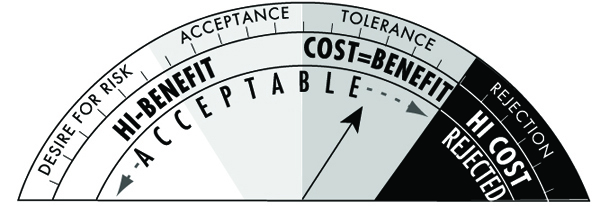
\includegraphics[width = 0.9\textwidth]{figure/risk.jpg}
    %\caption{Awesome figure}
  \end{figure}
\end{frame}

\begin{frame}{All eggs in one basket?}
  \begin{figure}
    \centering
    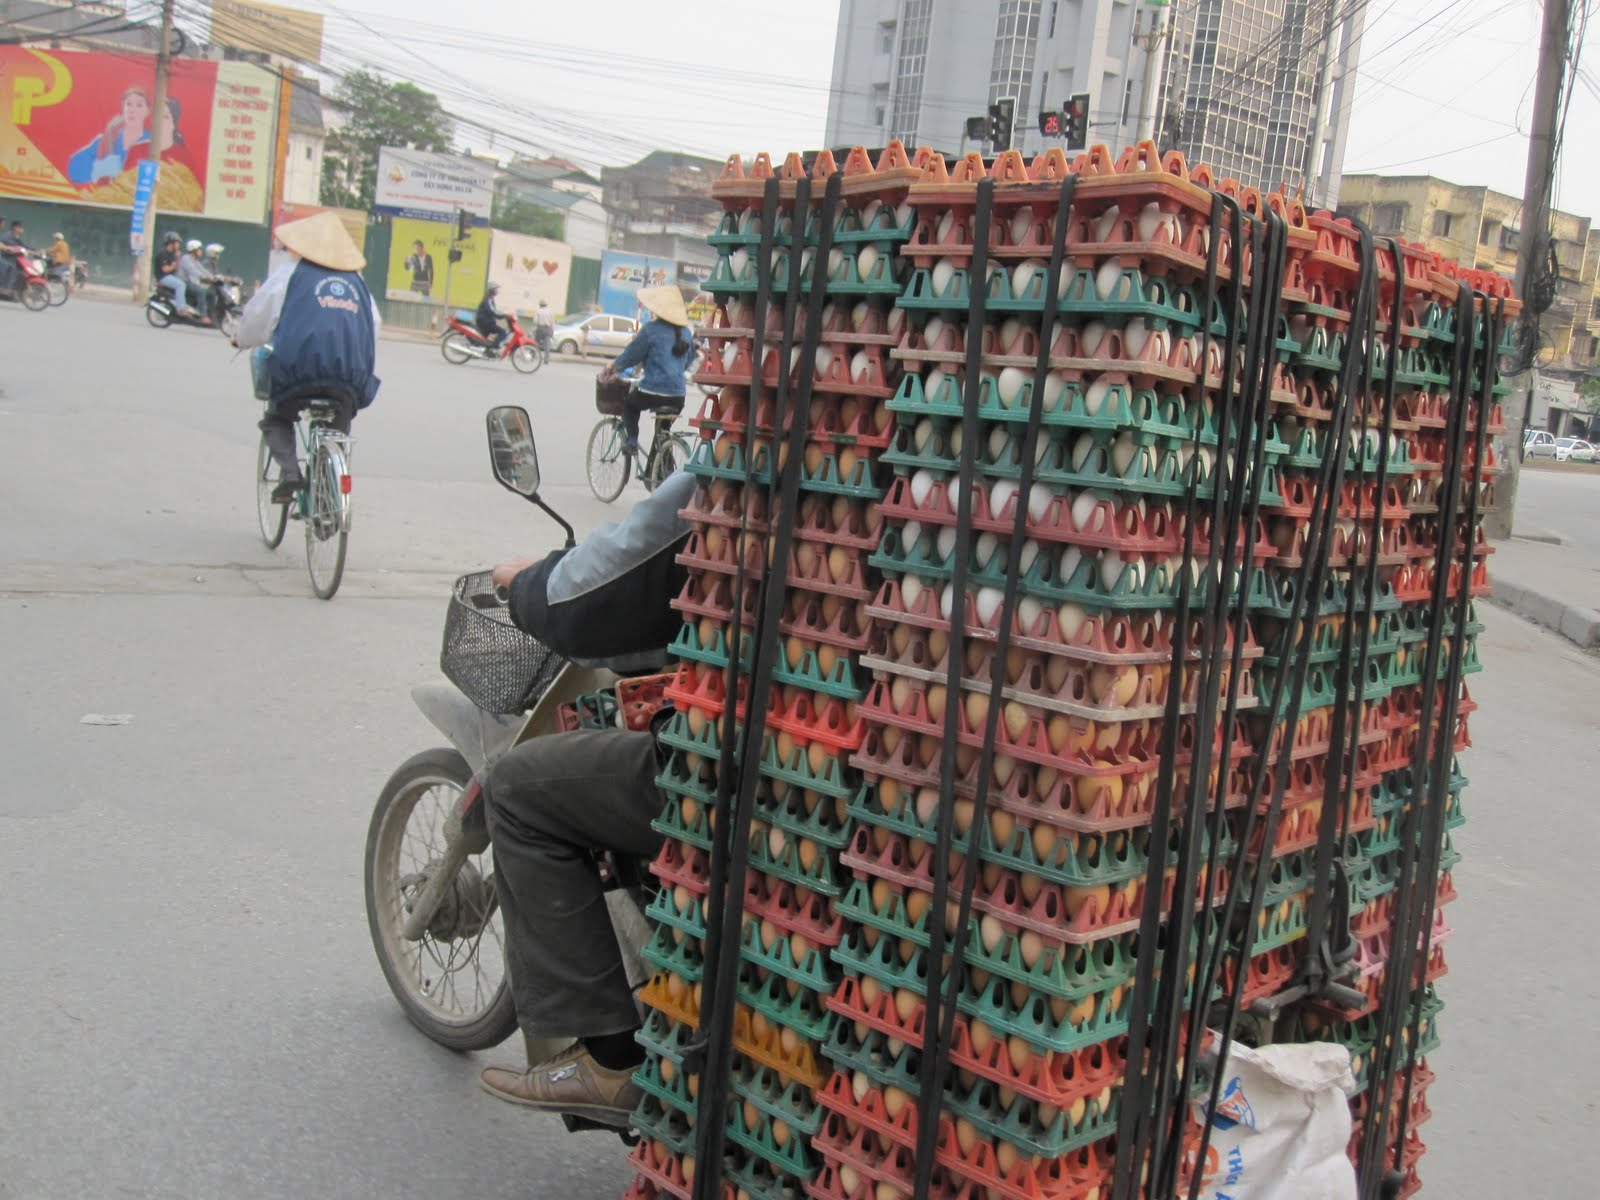
\includegraphics[width = 0.9\textwidth]{figure/alleggs.jpg}
    %\caption{Awesome figure}
  \end{figure}
\end{frame}

\begin{frame}{Diversifaction}
  \begin{figure}
    \centering
    
\includegraphics[width = 0.9\textwidth]{figure/allegg2.png}
    %\caption{Awesome figure}
  \end{figure}
\end{frame}

\begin{frame}{Portfolio Optimisation}
  \begin{figure}
    \centering
    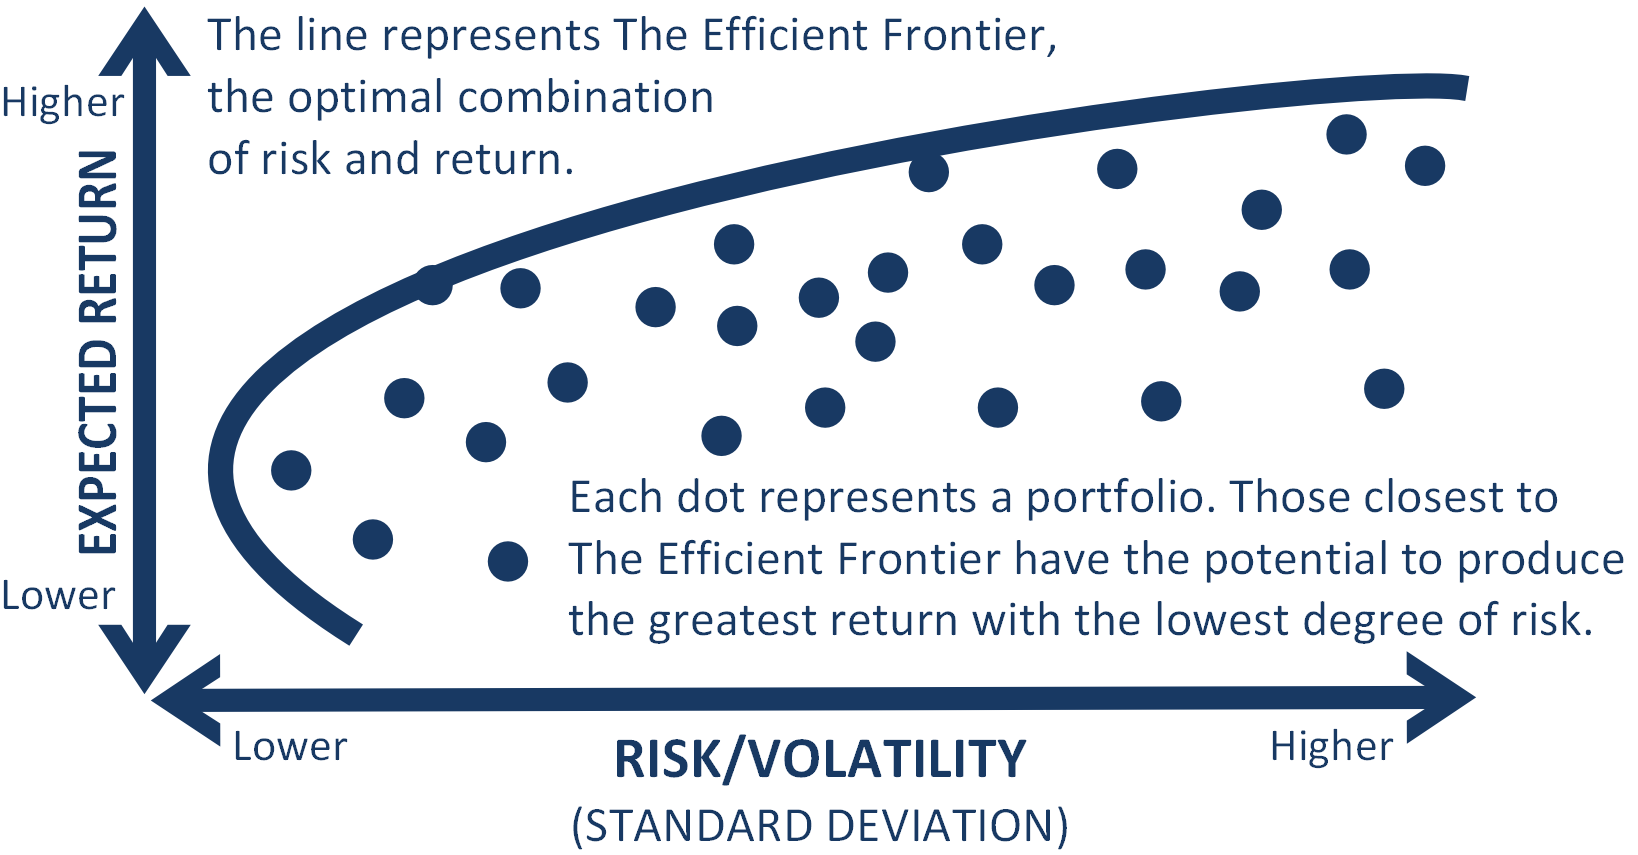
\includegraphics[width = 0.9\textwidth]{figure/mpt.png}
    %\caption{Awesome figure}
  \end{figure}
\end{frame}

\begin{frame}{A tale of two investment styles}

  \begin{figure}
    \centering
    \includegraphics[width = 0.7\textwidth]{figure/ap.jpg}
    %\caption{Awesome figure}
  \end{figure}
\end{frame}

\begin{frame}{S\&P Index for the last 5 Year}

  \begin{figure}
    \centering
    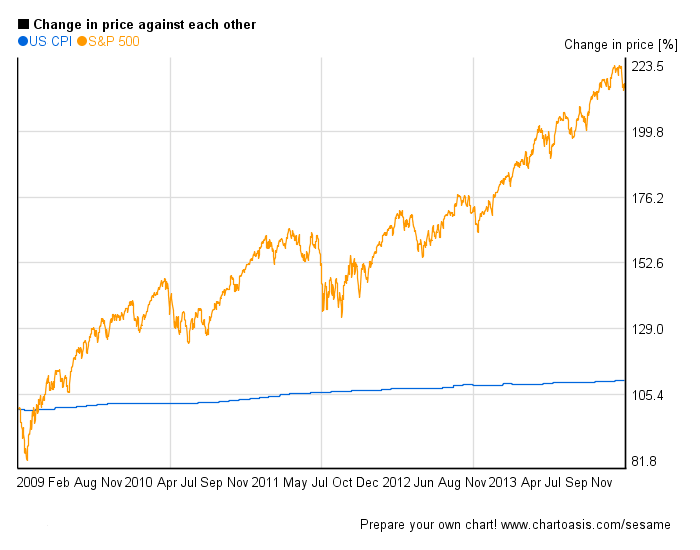
\includegraphics[width = 0.9\textwidth]{figure/snp500.png}
    %\caption{Awesome figure}
  \end{figure}

\end{frame}

\begin{frame}{Passive Index Fund}
   \begin{figure}
    \centering
    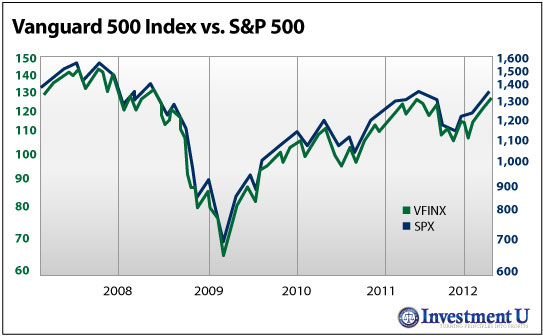
\includegraphics[width = 0.9\textwidth]{figure/vanguard.jpg}
    %\caption{Awesome figure}
  \end{figure}
\end{frame}

\begin{frame}{Why Index Fund?}
   \begin{enumerate}
\item Lower fees
\item Less vulnerable to the change of managers
\item Typically more tax efficient
\item Comparable performance?
   \end{enumerate}
\begin{block}{Objective}
Minimising the tracking error, $\epsilon$ of index tracking fund:
\begin{equation}
\epsilon = \sqrt{Var[r_p - r_b]}
\end{equation}
where $r_p$ is the return of the fund and $r_b$ is the return of the benchmark index.
\end{block}
\end{frame}

\begin{frame}{Methodology}
\begin{block}{State Space Model}
Adopt a conditional linear Gaussian Model
\begin{align*}
  X_t &= A_t(U_t)X_{t-1} + B_t(U_t)W_t + F_t(U_t) \nonumber \\
  Y_t &= C_t(U_t)X_t + D_t(U_t)V_t + G_t(U_t)
\label{eq:model}
\end{align*}
where $W_t, V_t \sim \mathcal{N}(0,I)$.
\end{block}

\begin{block}{Trasition Density and Conditional Likelihood}
\begin{align}
  p_t(u_t \mid u_{t-1}) &= \textrm{(any given form)} \nonumber \\
  f_t(x_t \mid x_{t-1}, u_t) &= \mathcal{N}(A_t(u_t) x_{t-1} + F_t(u_t), B_t(u_t)B_t(u_t)^T) \nonumber \\
  g_t(y_t \mid x_t, u_t)    &= \mathcal{N}(C_t(u_t) x_t + G_t(u_t), D_t(u_t)D_t(u_t)^T)
\end{align}
\end{block}
\end{frame}

\begin{frame}
\begin{block}{Open loop problem regulation}
Viewing portfolio optimisation as a stochastic control problem.
Express performance using a reward (cost function) $J_{x_0}(u_{1:T})$, where $J_{x_0}(u_{1:T})$ is an expectation of some function
\begin{equation}
  J(u_{1:T},y^{ref}_{1:T}, x_0) =E_{x_0}\left[\exp\left( -\dfrac{1}{2}\displaystyle\sum^T_{t=1}\left(\vert\vert y^{ref}_t - C_t(u_t)x_t - G_t(u_t) \vert\vert^2_{Q_t(u_t)^{-1}}  + \vert\vert u_t - u_{t-1} \vert\vert^2_{L_t}\right) \right) \right]
\end{equation}
where $Q(u_t) = D_t(u_t)D_t(u_t)^T$ and $L_t$ are assumed to known.
\end{block}
\end{frame}

\begin{frame}{Experiment 1: Tracking an oscillating wave}
\begin{block}{The state space model}
  $X_t = X_{t-1} + W_t + U_t, W_t \sim \mathcal{N}(0,I)$
  $Y_t = X_t + V_t, V_t \sim \mathcal{N}(0,I)$
\end{block}

\begin{block}{Target reference signal}
$y^{ref}_t = \cos(0.2 \pi t + 0.3)$ 
\end{block}

\begin{block}{Parameter Settings}
\begin{enumerate}
\item Various time period length, $T$: 5, 10 and 20.
\item Various sample size, $N$: 100, 500, 1000, 5000 and 10000.
\item Resampling step: Always vs. Selectively with ES.
\item Resample-Move step with MCMC (random walk proposal).
\item Various $\gamma$ settings: Constant function of $1$, $50$, $100$, $1000$ and increasing function of time $t$, $10t$, $50t$ and $100t$.
\end{enumerate}
\end{block}
\end{frame}

\begin{frame}{Experiment 1: Results and Discussion}
\begin{block}{Result and Discussion}
\begin{enumerate}
\item More samples helps --- better distribution representation
\item ESS doesn't help --- resampling pushes samples towards the mode
\item MCMC helps --- pertubation helps to escape local optimal
\item $\gamma$ setting need tuning --- optimisation vs. exploration
\end{enumerate}
\end{block}

  \begin{figure}
    \centering
    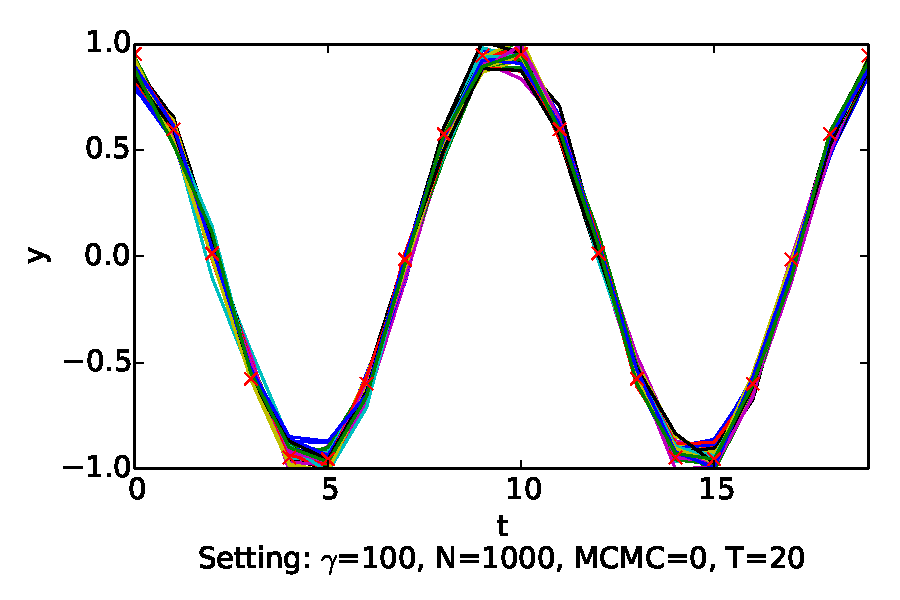
\includegraphics[width = 0.6\textwidth]{figure/output_y/output_20_100.pdf}
    %\caption{Awesome figure}
  \end{figure}
\end{frame}

\begin{frame}{Application: Tracking the DAX Index}
\begin{block}{the DAX Index}
\begin{enumerate}
\item One of the major index of the world
\item 30 largest companies in Germany as the constituents
\item Data: Adjusted daily close from Jan 2014
\end{enumerate}
\end{block}
\begin{block}{Experiments}
\begin{enumerate}
\item DAX4
\item DAX with full replication
\item DAX with partial replication
\item DAX with MPC
\end{enumerate}
\end{block}
\end{frame}

\begin{frame}{Experiment: Tracking the DAX Index}
\begin{block}{The state space model}
\begin{align*}
  X_t &= X_{t-1} + F_t(U_t) + W_t \\
  Y_t &= 30U^T_tX_t + 0.01V_t
\end{align*}
iwhere $W_t \sim \mathcal{N}(\mu_{t_0}, \Sigma_{t_0})$, $V_t \sim \mathcal{N}(0, I)$, $\{X_t\}_{t \geq 0}$ is a vector of stock price processes modelled as Arithmetic Brownian Motion with drift, $\{U_t\}_{t \geq 0}$ is a vector of control input processes, each component represents the position we have for each stock, $F_t(U_t)$ can be viewed as the market impact on price due to position changes and is set to be $0.0001U_t$ here, $\mu_{t_0}$ and $\Sigma_{t_0}$ are vector of the estimated mean of price changes and the estimated covariance matrix of the price changes and $\{Y_t\}_{t \geq 0}$ is the process represents the index level.
\end{block}
\end{frame}

\begin{frame}{Experiment 3:Full Replication}
   \begin{figure}
    \centering
    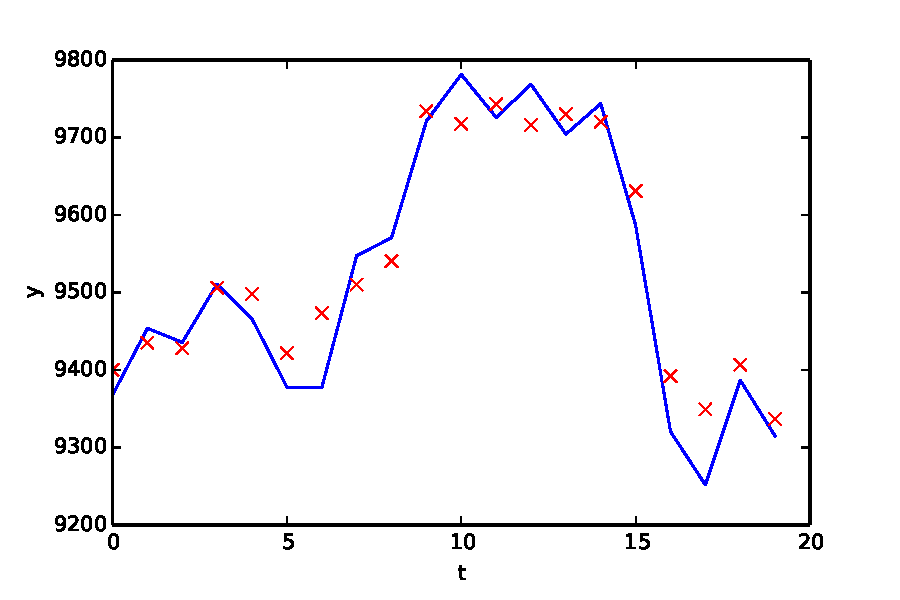
\includegraphics[width = 0.9\textwidth, height=0.4\textheight]{figure/DAXFull-y.pdf}\\
    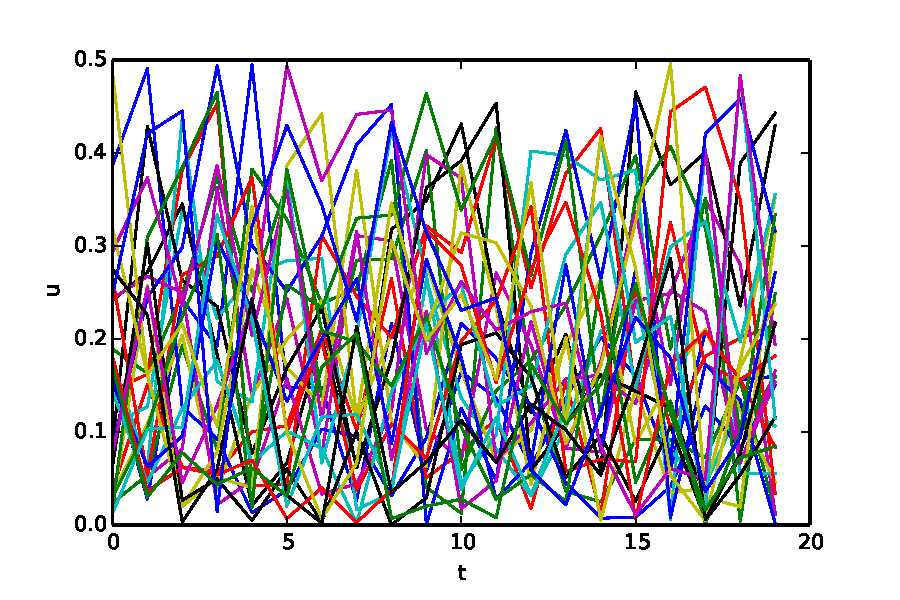
\includegraphics[width = 0.9\textwidth, height=0.4\textheight]{figure/DAXFull-u.pdf}
   \end{figure}
\end{frame}


\begin{frame}{Experiment 3:Partial Replication}
   \begin{figure}
    \centering
    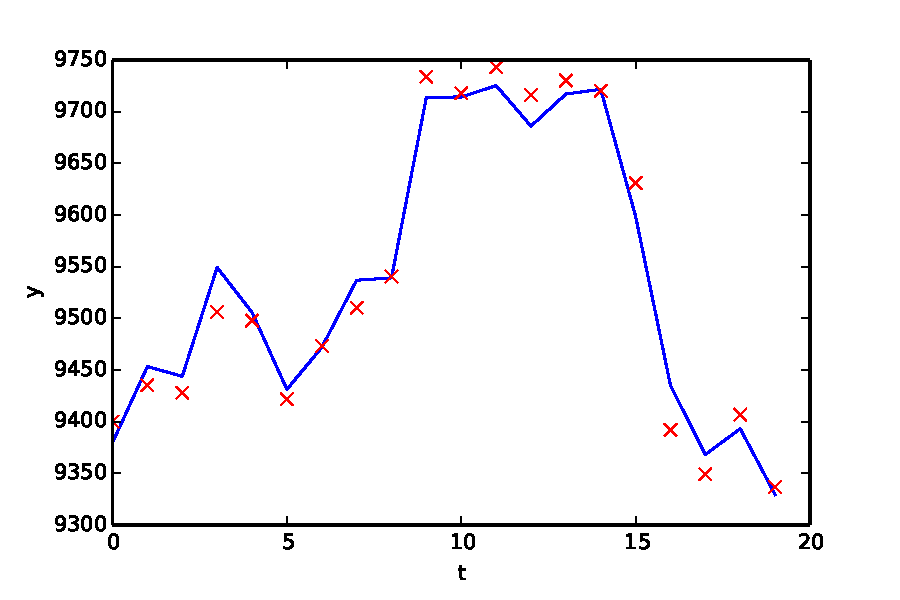
\includegraphics[width = 0.9\textwidth, height=0.4\textheight]{figure/DAXPartial-y.pdf}\\
    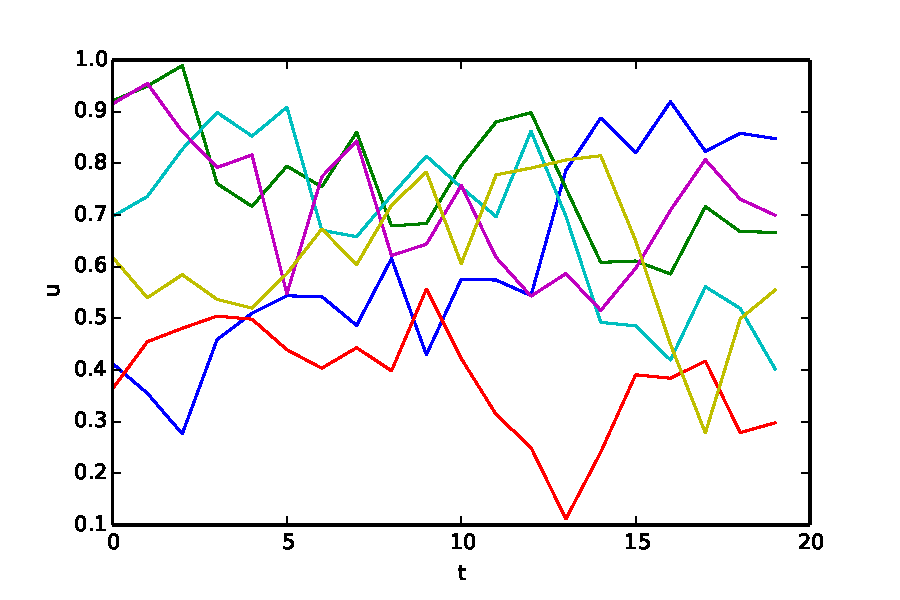
\includegraphics[width = 0.9\textwidth, height=0.4\textheight]{figure/DAXPartial-u.pdf}
	\end{figure}
\end{frame}


\begin{frame}{What we have achieved so far}
\begin{block}{What the technique can do?}
Track a \emph{given} target reference index.
\end{block}

\begin{block}{Issues}
\begin{enumerate}
\item We do not have a reference signal
\item Open loop policy, no feedback used
\end{enumerate}
\end{block}

\begin{block}{Solution}
\begin{enumerate}
\item use EWMA estimate for the target reference signal
\item use Model Predictive Control (MPC)
\end{enumerate}
\end{block}
\end{frame}

\begin{frame}{MPC: Algorithm}
  \begin{algorithmic}[1]
  \Function{ModelPredictiveControl}{T,H}
  \State Set $t = 1$.
  \While{$t \leq T$}
  \State Search the optimal $u^*_{t:t+H}$ for the problem $t:t+H$.
  \State Apply the first set of the optimal control  $u^*_{t}$.
  \State Update the model states with any new information.
  \State Set $t = t + 1$.
  \EndWhile
  \EndFunction
  \end{algorithmic}
\end{frame}

\begin{frame}{MPC: Results and Discussion}

   \begin{figure}
    \centering
    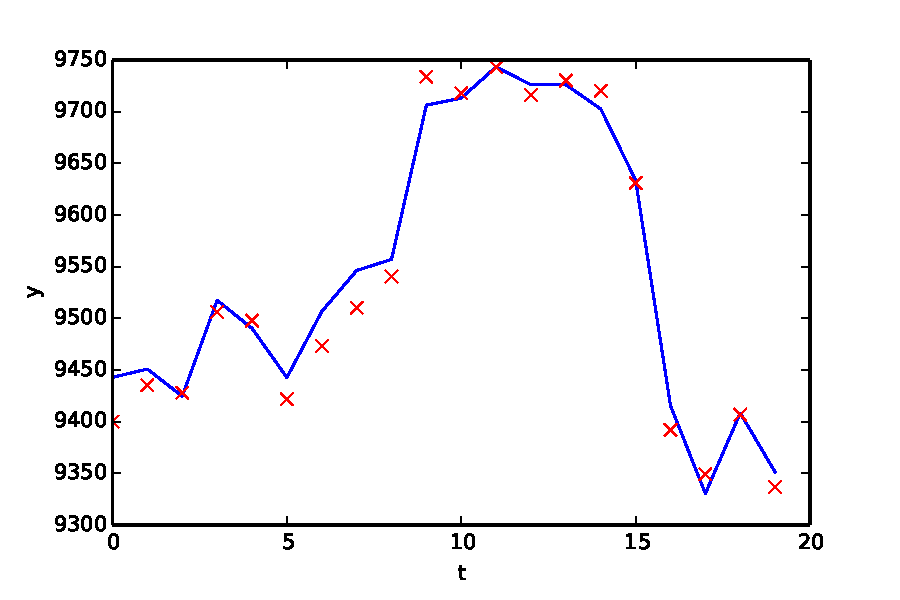
\includegraphics[width = 0.9\textwidth, height=0.4\textheight]{figure/DAXMPC-y-2.pdf}\\
    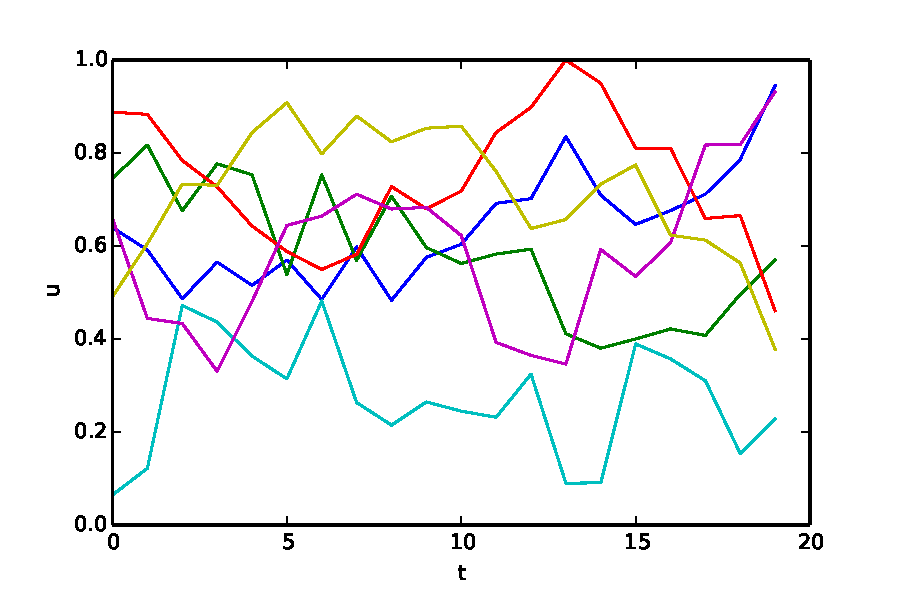
\includegraphics[width = 0.9\textwidth, height=0.4\textheight]{figure/DAXMPC-u-2.pdf}
  \end{figure}
\end{frame}


\begin{frame}{MPC: Results and Discussion}

   \begin{figure}
    \centering
    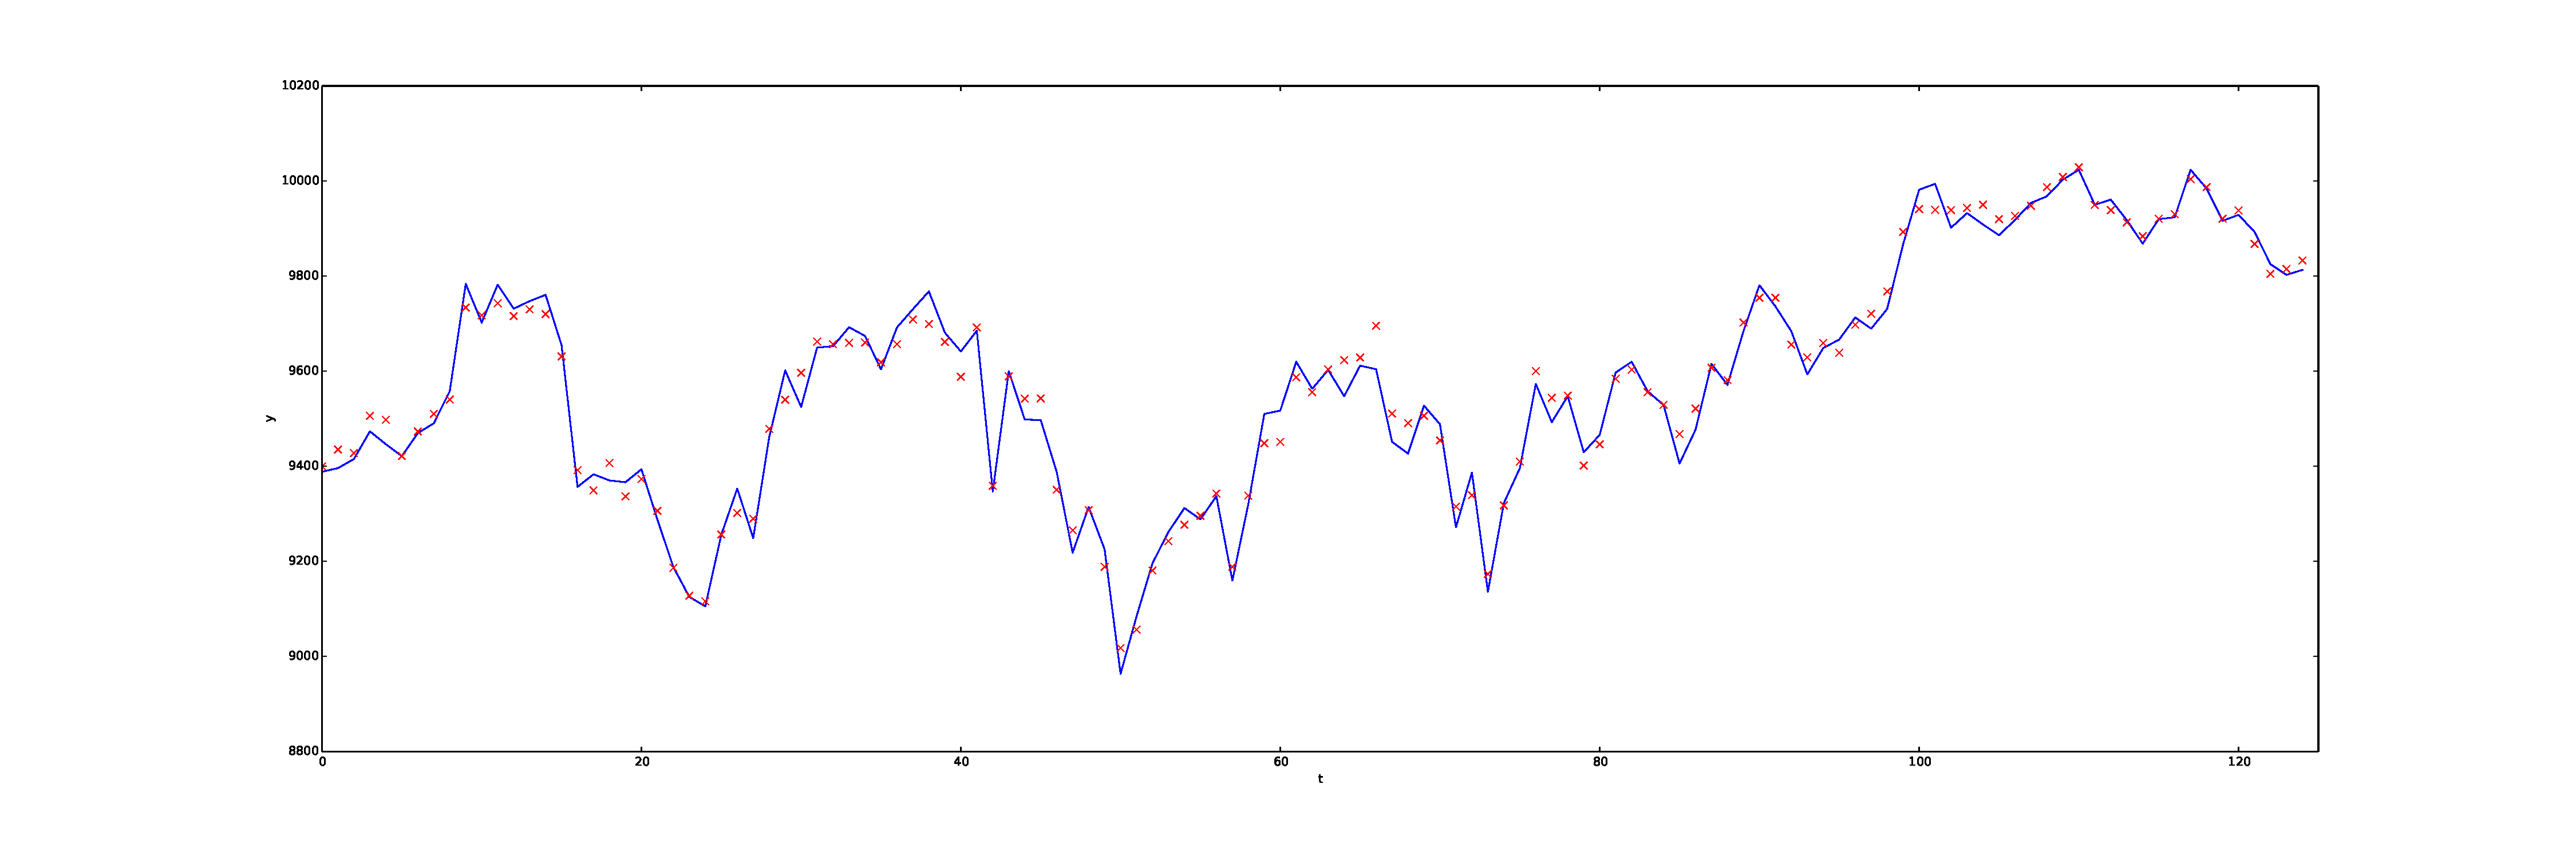
\includegraphics[width = 0.9\textwidth, height=0.4\textheight]{figure/DAXMPC-y-2-long.pdf}\\
    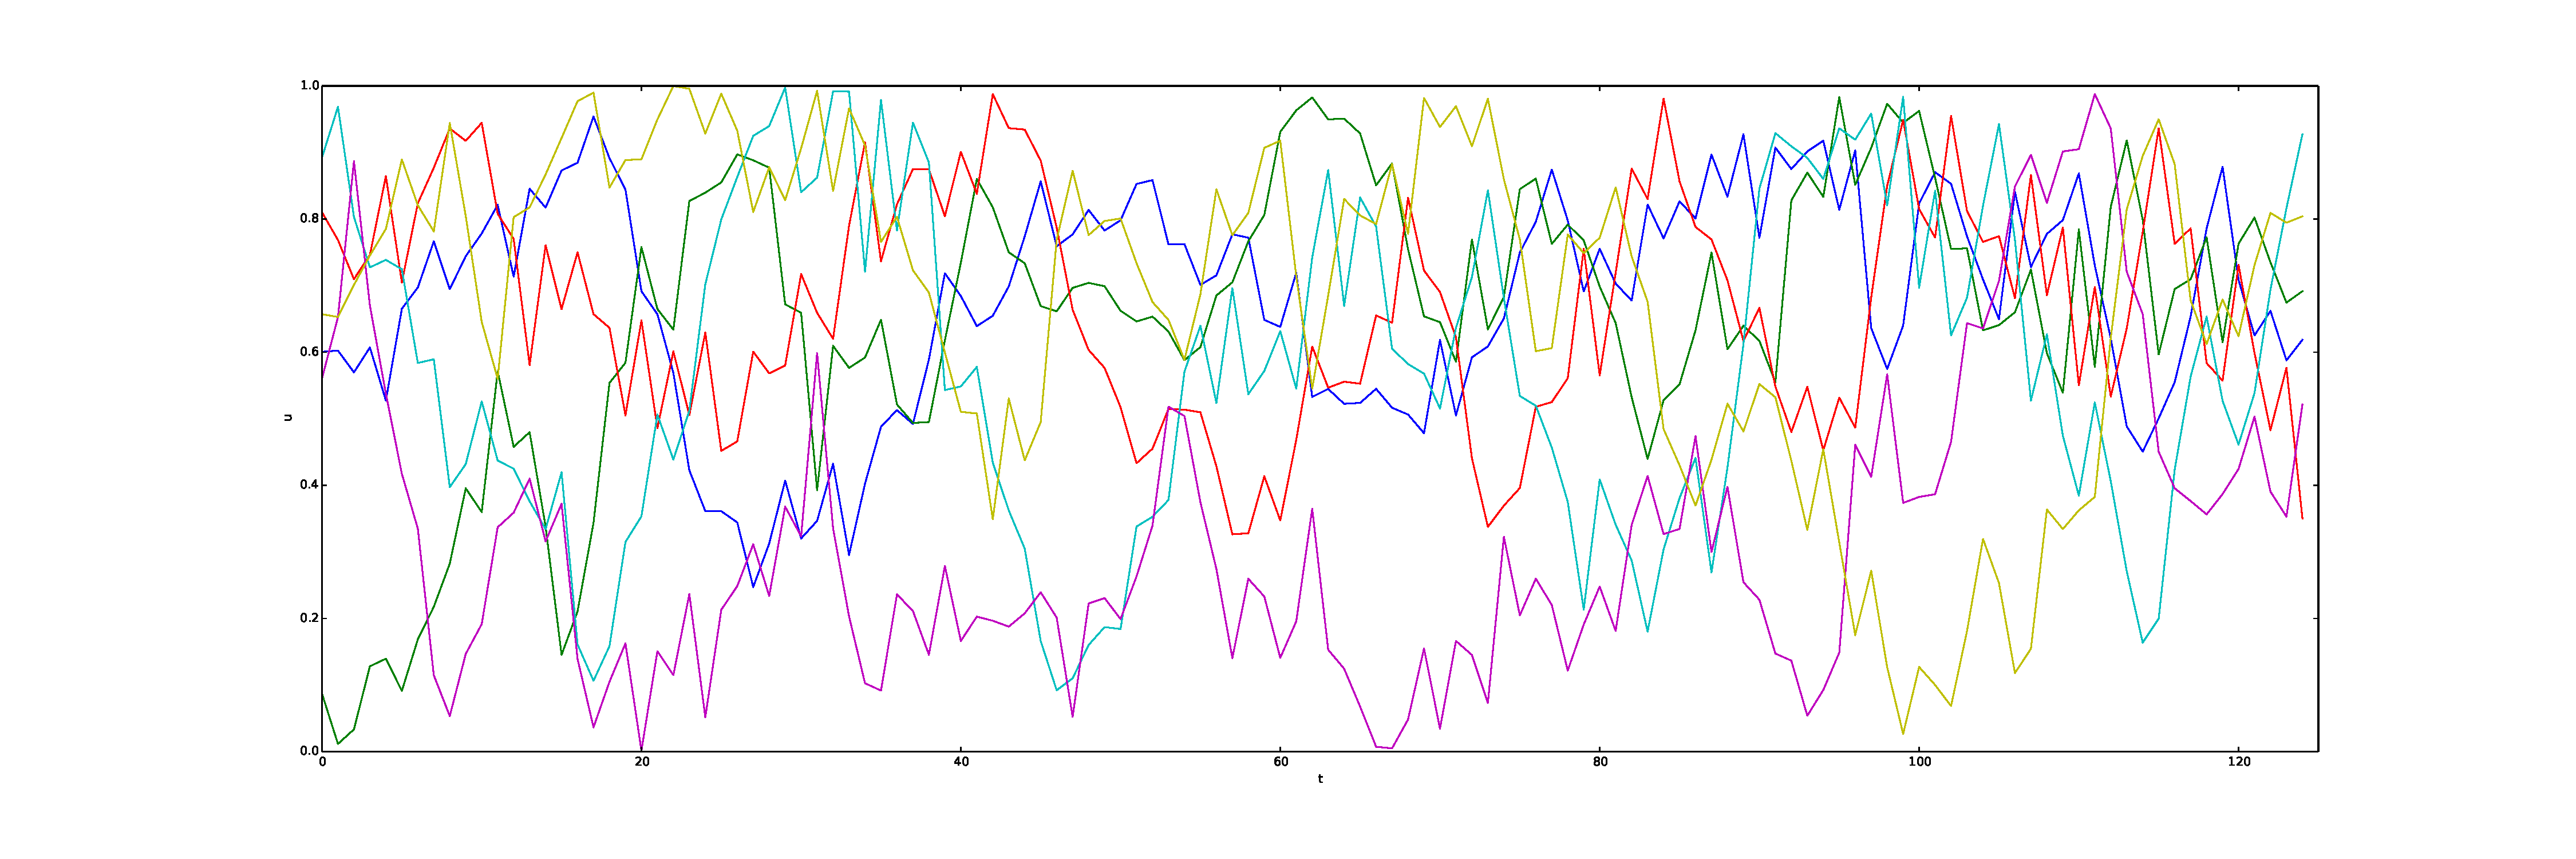
\includegraphics[width = 0.9\textwidth, height=0.4\textheight]{figure/DAXMPC-u-2-long.pdf}
  \end{figure}
\end{frame}

\section{Conclusions}
\begin{frame}{Contributions}
In this thesis, it is found that SMC has the potential to be an effective means of searching the optimal strategy for index tracking funds. The following work has been carried out:
\begin{enumerate}
\item exploring the potential of SMC in searching the optimal strategy for minimising the tracking error and transaction costs of an index fund. 
\item exploring the sensitivity of SMC in terms of the parameter settings, the trade-off between estimation accuracy and computational efforts numerically and providing suggestions for real-world problem.
\item introducing the Model Predictive Control (MPC) framework and demonstrate how to integrate SMC technique proposed into the MPC framework.
\end{enumerate}
\end{frame}

\begin{frame}{Future Work}
\begin{enumerate}
\item More realistic models
  \begin{itemize}
   \item Geometric Brownian Model, Jump Diffusion model, etc.
   \item Moving away from a conditional Gaussian model \\$\implies$ the  Kalman Filter recursion is no longer optimal.
   \item Try: SMC2.
  \end{itemize}
\item Parallel computation --- The nested SMC setup inevitably adds consideration amount of computation requirements. 

\item More complex financial indices
\end{enumerate}
\end{frame}

\begin{frame}{Questions?}
Thank you.
\end{frame}


\end{document}
